\documentclass[10pt,a4paper,landscape]{report}
\usepackage[dutch]{babel}
\usepackage{amsmath}
\usepackage{amsfonts}
\usepackage{amssymb}
\usepackage{graphicx}
\usepackage{tikz}
\usepackage{environ}
\makeatletter
\newsavebox{\measure@tikzpicture}
\NewEnviron{scaletikzpicturetowidth}[1]{%
  \def\tikz@width{#1}%
  \def\tikzscale{1}\begin{lrbox}{\measure@tikzpicture}%
  \BODY
  \end{lrbox}%
  \pgfmathparse{#1/\wd\measure@tikzpicture}%
  \edef\tikzscale{\pgfmathresult}%
  \BODY
}
\makeatother
\usepackage[left=2cm,right=2cm,top=3cm,bottom=3cm]{geometry}
\author{Aranka Steyaert}
\begin{document}
\begin{scaletikzpicturetowidth}{\linewidth}
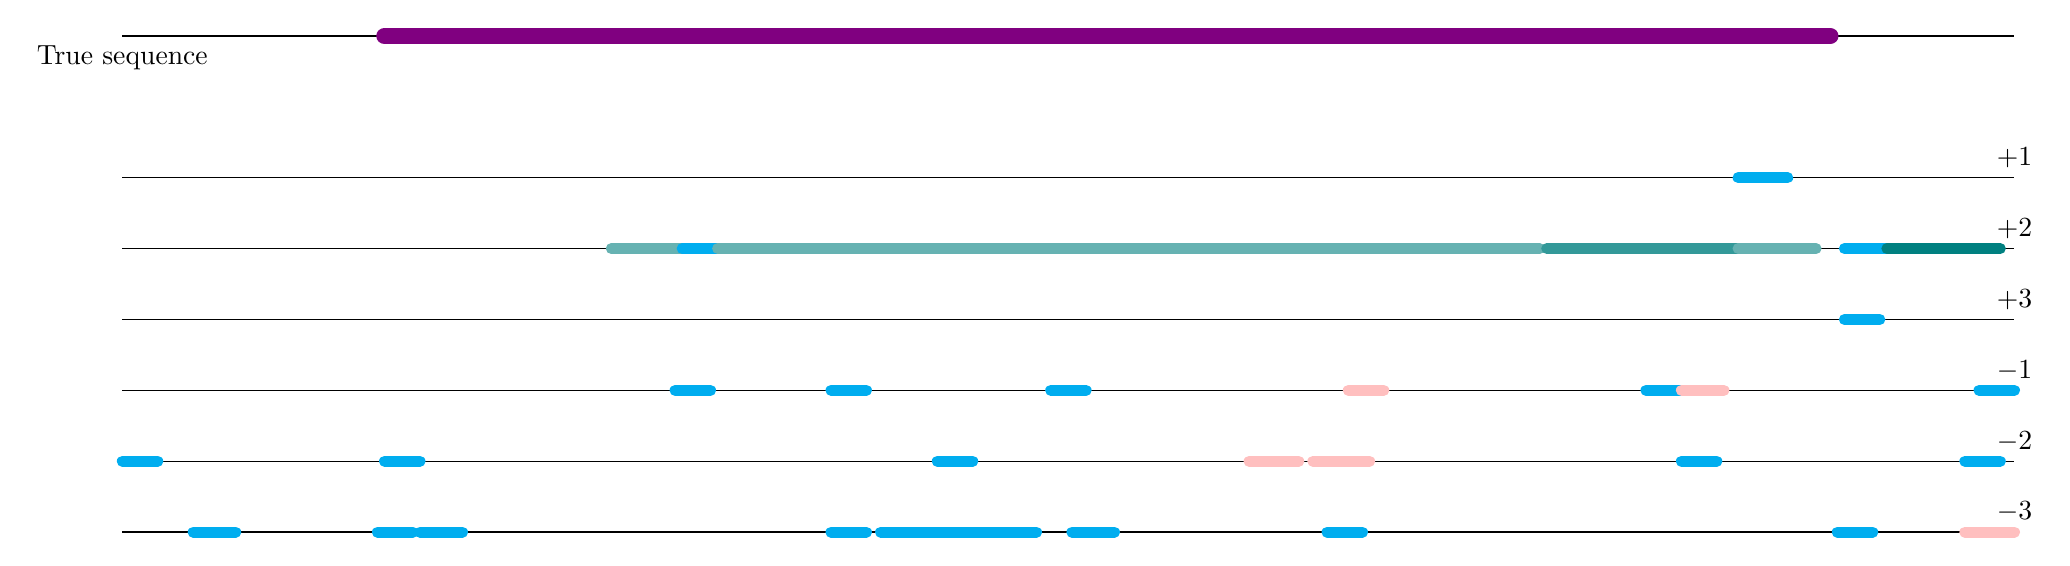
\begin{tikzpicture}
[scale=0.9,
root/.style={cyan, line width = 4pt, line cap = round},
genus/.style={teal!60, line width = 4pt, line cap = round},
species/.style={teal, line width = 4pt, line cap = round},
species group/.style={teal!80, line width = 4pt, line cap = round},
wrong/.style={pink, line width = 4pt, line cap = round},
superkingdom/.style={teal!10, line width = 4pt, line cap = round}]
\draw node[anchor=north] {True sequence} (0,0) -- (26.7,0) ;
\draw (0,-2) -- (26.7,-2) node[anchor=south] {$+1$};
\draw (0,-3) -- (26.7,-3) node[anchor=south] {$+2$};
\draw (0,-4) -- (26.7,-4) node[anchor=south] {$+3$};
\draw (0,-5) -- (26.7,-5) node[anchor=south] {$-1$};
\draw (0,-6) -- (26.7,-6) node[anchor=south] {$-2$};
\draw (0,-7) -- (26.7,-7) node[anchor=south] {$-3$};
\draw[violet, line width = 6pt, line cap = round] (3.7,0) -- (24.1,0);
\draw[root] (22.8,-2) -- (23.5,-2);
\draw[genus] (6.9,-3)--(7.9,-3);
\draw[root] (7.9,-3)--(8.4,-3);
\draw[genus] (8.4,-3)--(11.7,-3);
\draw[genus] (11.7,-3)--(14.5,-3);
\draw[genus] (14.5,-3)--(17.3,-3);
\draw[genus] (17.3,-3)--(20,-3);
\draw[species group] (20.1,-3)--(22.8,-3);
\draw[genus] (22.8,-3)--(23.9,-3);
\draw[root] (24.3,-3)--(24.9,-3);
\draw[species] (24.9,-3)--(26.5,-3);
\draw[root] (24.3,-4)--(24.8,-4);
\draw[root] (7.8,-5)--(8.3,-5);
\draw[root] (10,-5)--(10.5,-5);
\draw[root] (13.1,-5)--(13.6,-5);
\draw[wrong] (17.3,-5)--(17.8,-5);
\draw[root] (21.5,-5)--(22,-5);
\draw[wrong] (22,-5)--(22.6,-5);
\draw[root] (26.2,-5)--(26.7,-5);
\draw[root] (0,-6)--(0.5,-6);
\draw[root] (3.7,-6)--(4.2,-6);
\draw[root] (11.5,-6)--(12,-6);
\draw[wrong] (15.9,-6)--(16.6,-6);
\draw[wrong] (16.8,-6)--(17.6,-6);
\draw[root] (22,-6)--(22.5,-6);
\draw[root] (26,-6)--(26.5,-6);
\draw[root] (1,-7)--(1.6,-7);
\draw[root] (3.6,-7)--(4.1,-7);
\draw[root] (4.2,-7)--(4.8,-7);
\draw[root] (10,-7)--(10.5,-7);
\draw[root] (10.7,-7)--(11.4,-7);
\draw[root] (11.4,-7)--(11.9,-7);
\draw[root] (11.9,-7)--(12.4,-7);
\draw[root] (12.4,-7)--(12.9,-7);
\draw[root] (13.4,-7)--(14,-7);
\draw[root] (17,-7)--(17.5,-7);
\draw[root] (24.2,-7)--(24.7,-7);
\draw[wrong] (26,-7)--(26.7,-7);
\end{tikzpicture}
\end{scaletikzpicturetowidth}
\vspace{2cm}
\begin{scaletikzpicturetowidth}{\linewidth}
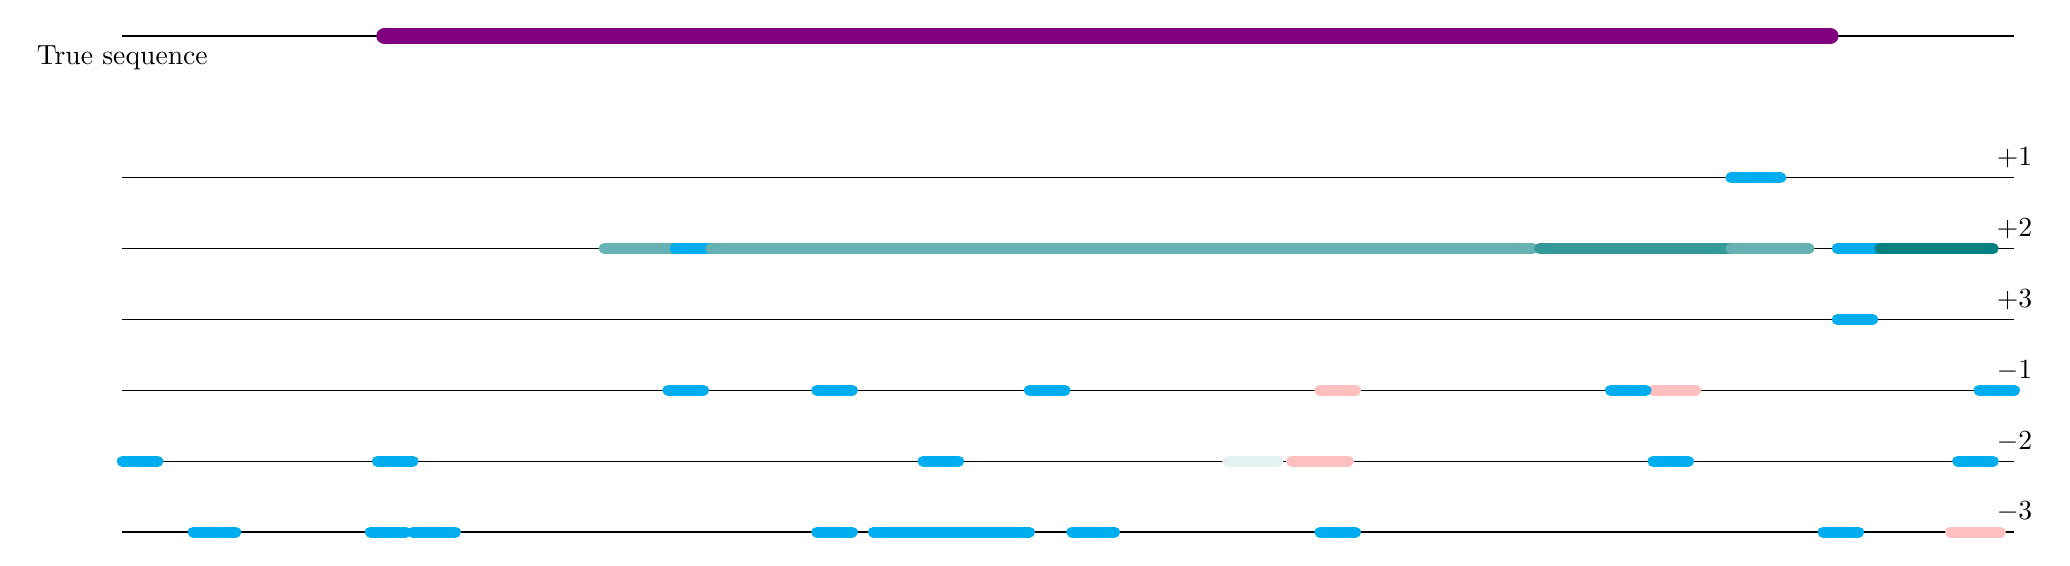
\begin{tikzpicture}
[scale=0.9,
root/.style={cyan, line width = 4pt, line cap = round},
genus/.style={teal!60, line width = 4pt, line cap = round},
species/.style={teal, line width = 4pt, line cap = round},
species group/.style={teal!80, line width = 4pt, line cap = round},
wrong/.style={pink, line width = 4pt, line cap = round},
superkingdom/.style={teal!10, line width = 4pt, line cap = round}]
\draw node[anchor=north] {True sequence} (0,0) -- (26.7,0) ;
\draw (0,-2) -- (26.7,-2) node[anchor=south] {$+1$};
\draw (0,-3) -- (26.7,-3) node[anchor=south] {$+2$};
\draw (0,-4) -- (26.7,-4) node[anchor=south] {$+3$};
\draw (0,-5) -- (26.7,-5) node[anchor=south] {$-1$};
\draw (0,-6) -- (26.7,-6) node[anchor=south] {$-2$};
\draw (0,-7) -- (26.7,-7) node[anchor=south] {$-3$};
\draw[violet, line width = 6pt, line cap = round] (3.7,0) -- (24.1,0);
\draw[root] (22.7,-2) -- (23.4,-2);
\draw[genus] (6.8,-3) -- (7.8,-3);
\draw[root] (7.8,-3) -- (8.3,-3);
\draw[genus] (8.3,-3) -- (11.600000000000001,-3);
\draw[genus] (11.6,-3) -- (14.399999999999999,-3);
\draw[genus] (14.4,-3) -- (17.2,-3);
\draw[genus] (17.2,-3) -- (19.9,-3);
\draw[species group] (20.0,-3) -- (22.7,-3);
\draw[genus] (22.7,-3) -- (23.8,-3);
\draw[root] (24.2,-3) -- (24.8,-3);
\draw[species] (24.8,-3) -- (26.400000000000002,-3);
\draw[root] (24.2,-4) -- (24.7,-4);
\draw[root] (26.2,-5) -- (26.7,-5);
\draw[wrong] (21.599999999999998,-5) -- (22.2,-5);
\draw[root] (21.0,-5) -- (21.5,-5);
\draw[wrong] (16.9,-5) -- (17.4,-5);
\draw[root] (12.799999999999999,-5) -- (13.299999999999999,-5);
\draw[root] (9.8,-5) -- (10.3,-5);
\draw[root] (7.699999999999999,-5) -- (8.2,-5);
\draw[root] (25.900000000000002,-6) -- (26.400000000000002,-6);
\draw[root] (21.6,-6) -- (22.1,-6);
\draw[wrong] (16.5,-6) -- (17.3,-6);
\draw[superkingdom] (15.600000000000001,-6) -- (16.3,-6);
\draw[root] (11.3,-6) -- (11.8,-6);
\draw[root] (3.6000000000000014,-6) -- (4.100000000000001,-6);
\draw[root] (0.0,-6) -- (0.5,-6);
\draw[wrong] (25.8,-7) -- (26.5,-7);
\draw[root] (24.0,-7) -- (24.5,-7);
\draw[root] (16.900000000000002,-7) -- (17.400000000000002,-7);
\draw[root] (13.400000000000002,-7) -- (14.000000000000002,-7);
\draw[root] (12.3,-7) -- (12.8,-7);
\draw[root] (11.8,-7) -- (12.3,-7);
\draw[root] (11.3,-7) -- (11.8,-7);
\draw[root] (10.600000000000001,-7) -- (11.3,-7);
\draw[root] (9.8,-7) -- (10.3,-7);
\draw[root] (4.100000000000003,-7) -- (4.700000000000003,-7);
\draw[root] (3.5,-7) -- (4.0,-7);
\draw[root] (1.0000000000000013,-7) -- (1.6000000000000014,-7);
\end{tikzpicture}
\end{scaletikzpicturetowidth}
\end{document}